% Options for packages loaded elsewhere
\PassOptionsToPackage{unicode}{hyperref}
\PassOptionsToPackage{hyphens}{url}
%
\documentclass[
  ignorenonframetext,
]{beamer}
\usepackage{pgfpages}
\setbeamertemplate{caption}[numbered]
\setbeamertemplate{caption label separator}{: }
\setbeamercolor{caption name}{fg=normal text.fg}
\beamertemplatenavigationsymbolsempty
% Prevent slide breaks in the middle of a paragraph
\widowpenalties 1 10000
\raggedbottom
\setbeamertemplate{part page}{
  \centering
  \begin{beamercolorbox}[sep=16pt,center]{part title}
    \usebeamerfont{part title}\insertpart\par
  \end{beamercolorbox}
}
\setbeamertemplate{section page}{
  \centering
  \begin{beamercolorbox}[sep=12pt,center]{part title}
    \usebeamerfont{section title}\insertsection\par
  \end{beamercolorbox}
}
\setbeamertemplate{subsection page}{
  \centering
  \begin{beamercolorbox}[sep=8pt,center]{part title}
    \usebeamerfont{subsection title}\insertsubsection\par
  \end{beamercolorbox}
}
\AtBeginPart{
  \frame{\partpage}
}
\AtBeginSection{
  \ifbibliography
  \else
    \frame{\sectionpage}
  \fi
}
\AtBeginSubsection{
  \frame{\subsectionpage}
}
\usepackage{lmodern}
\usepackage{amssymb,amsmath}
\usepackage{ifxetex,ifluatex}
\ifnum 0\ifxetex 1\fi\ifluatex 1\fi=0 % if pdftex
  \usepackage[T1]{fontenc}
  \usepackage[utf8]{inputenc}
  \usepackage{textcomp} % provide euro and other symbols
\else % if luatex or xetex
  \usepackage{unicode-math}
  \defaultfontfeatures{Scale=MatchLowercase}
  \defaultfontfeatures[\rmfamily]{Ligatures=TeX,Scale=1}
\fi
\usetheme[]{CambridgeUS}
% Use upquote if available, for straight quotes in verbatim environments
\IfFileExists{upquote.sty}{\usepackage{upquote}}{}
\IfFileExists{microtype.sty}{% use microtype if available
  \usepackage[]{microtype}
  \UseMicrotypeSet[protrusion]{basicmath} % disable protrusion for tt fonts
}{}
\makeatletter
\@ifundefined{KOMAClassName}{% if non-KOMA class
  \IfFileExists{parskip.sty}{%
    \usepackage{parskip}
  }{% else
    \setlength{\parindent}{0pt}
    \setlength{\parskip}{6pt plus 2pt minus 1pt}}
}{% if KOMA class
  \KOMAoptions{parskip=half}}
\makeatother
\usepackage{xcolor}
\IfFileExists{xurl.sty}{\usepackage{xurl}}{} % add URL line breaks if available
\IfFileExists{bookmark.sty}{\usepackage{bookmark}}{\usepackage{hyperref}}
\hypersetup{
  pdftitle={Comorbidities and COVID-19 in Mexico},
  pdfauthor={SJ McGeady; Esteban Fern'andez},
  hidelinks,
  pdfcreator={LaTeX via pandoc}}
\urlstyle{same} % disable monospaced font for URLs
\newif\ifbibliography
\usepackage{longtable,booktabs}
\usepackage{caption}
% Make caption package work with longtable
\makeatletter
\def\fnum@table{\tablename~\thetable}
\makeatother
\setlength{\emergencystretch}{3em} % prevent overfull lines
\providecommand{\tightlist}{%
  \setlength{\itemsep}{0pt}\setlength{\parskip}{0pt}}
\setcounter{secnumdepth}{-\maxdimen} % remove section numbering
\usepackage[font={small}, labelfont={bf}]{caption}

\title{Comorbidities and COVID-19 in Mexico}
\subtitle{A Comprehensive Data Analysis}
\author{SJ McGeady \and Esteban Fern\a'andez}
\date{July 2020}

\begin{document}
\frame{\titlepage}

\hypertarget{results}{%
\section{Results}\label{results}}

\hypertarget{logistic-regression}{%
\subsection{Logistic Regression}\label{logistic-regression}}

\begin{frame}{National-Level Findings}
\protect\hypertarget{national-level-findings}{}
\end{frame}

\begin{frame}{Odds-Ratios Plots}
\protect\hypertarget{odds-ratios-plots}{}
\begin{center}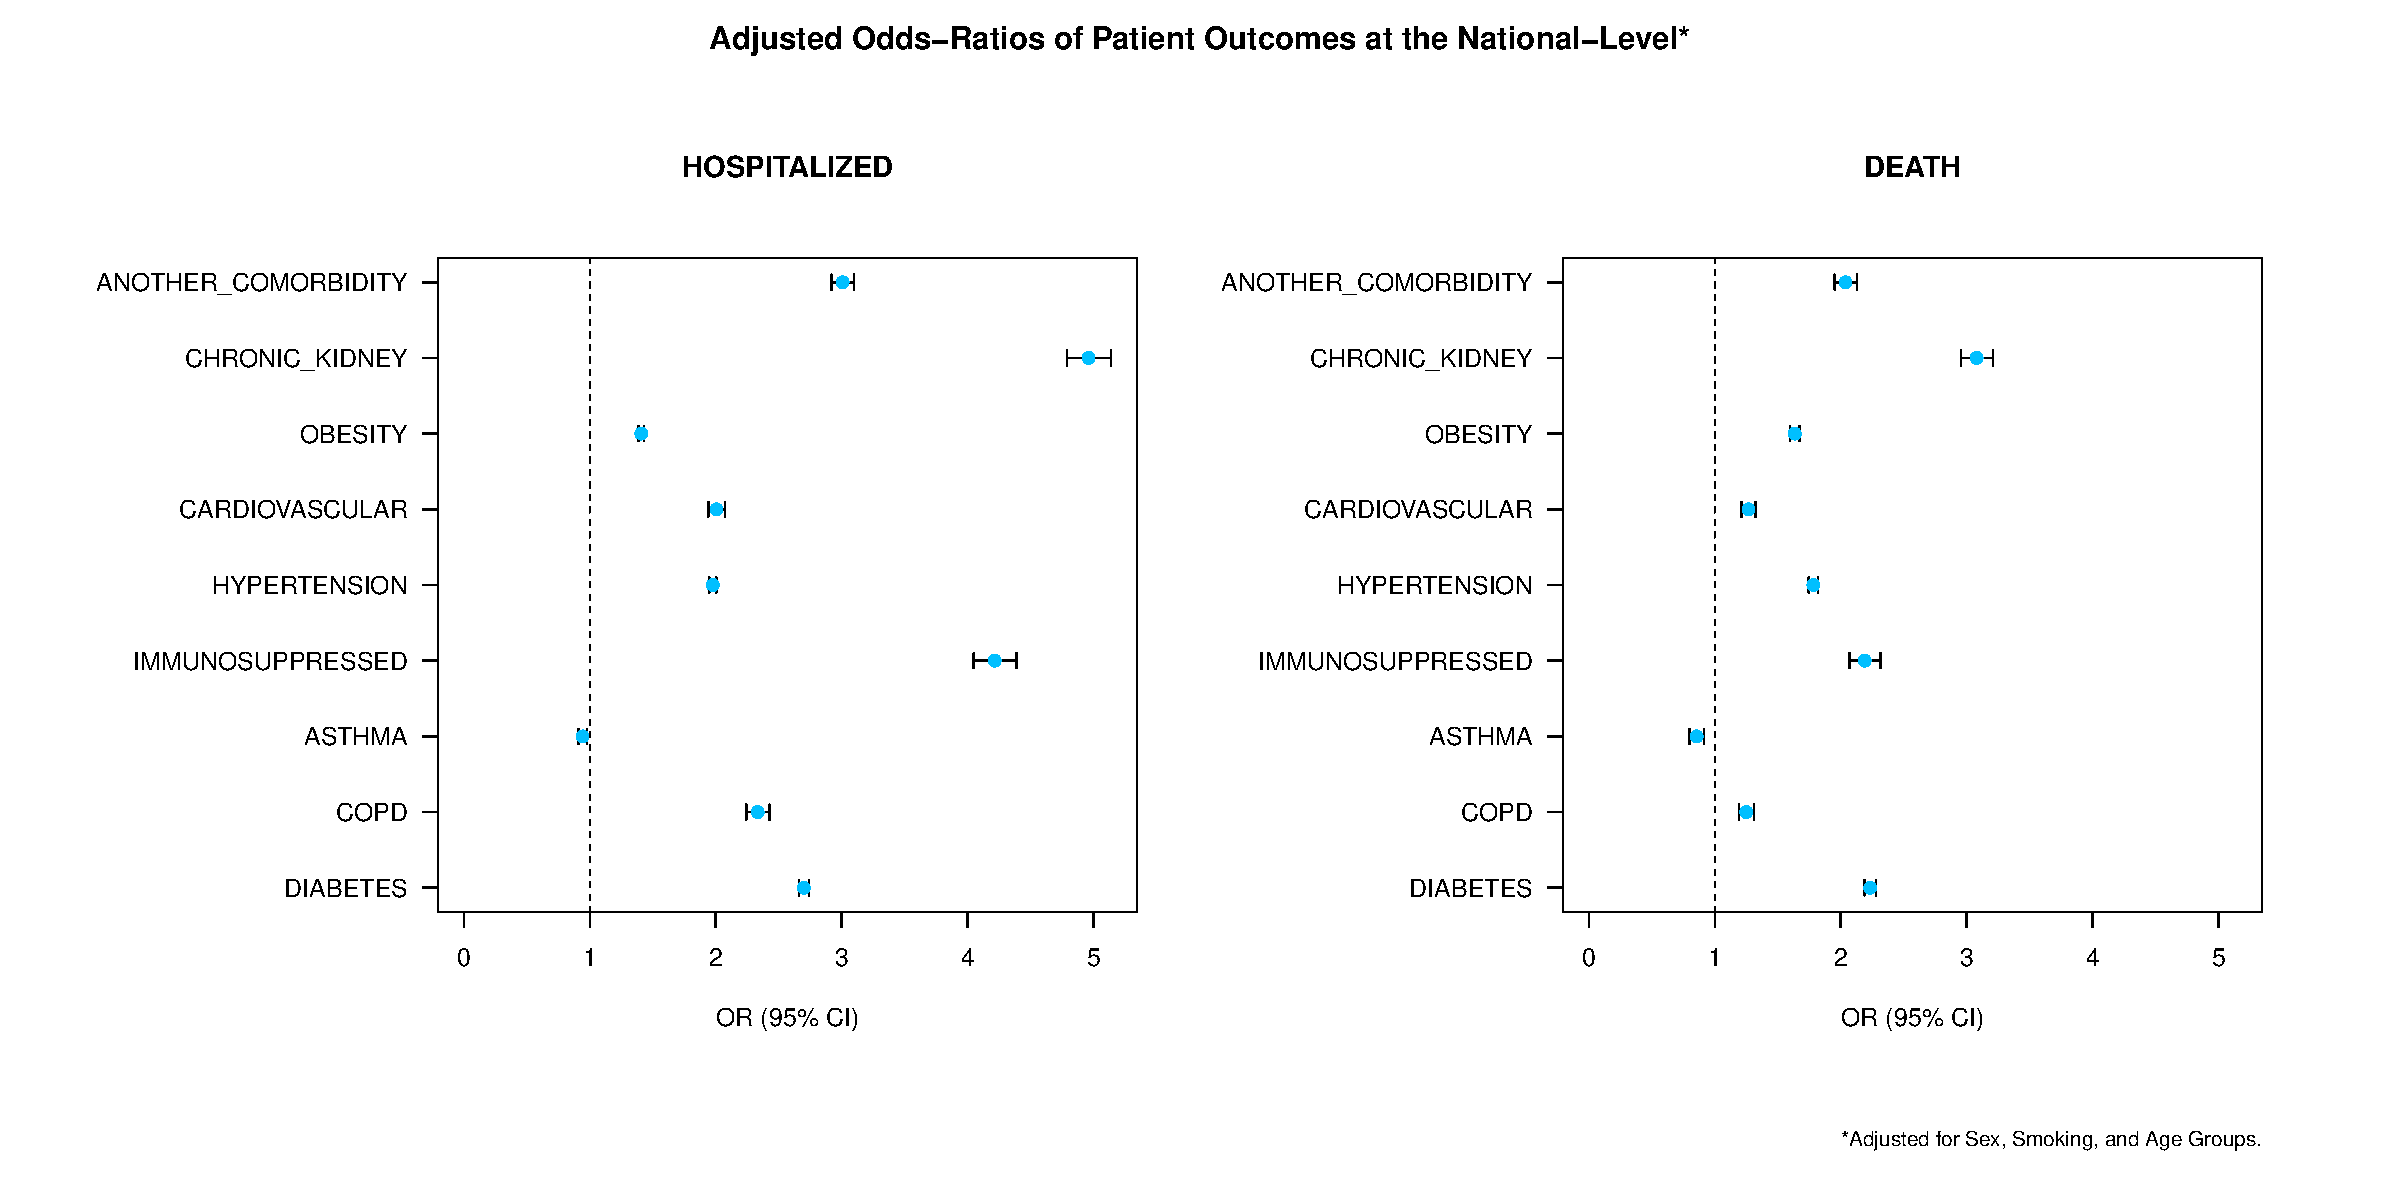
\includegraphics[width=1\linewidth]{/Users/estfernandez/Desktop/COVID-19 Comorbidities Data Analysis/figures/National_LR_Adjusted_Outcomes} \end{center}
\end{frame}

\begin{frame}{Odds-Ratios Table}
\protect\hypertarget{odds-ratios-table}{}
\begin{longtable}[]{@{}lrrrr@{}}
\caption{Odds-ratios table for Hospitalizations.}\tabularnewline
\toprule
& exp(coef) & lower .95 & upper .95 &
Pr(\textgreater\textbar z\textbar)\tabularnewline
\midrule
\endfirsthead
\toprule
& exp(coef) & lower .95 & upper .95 &
Pr(\textgreater\textbar z\textbar)\tabularnewline
\midrule
\endhead
DIABETES & 2.699 & 2.660 & 2.739 & 0.000\tabularnewline
COPD & 2.333 & 2.243 & 2.427 & 0.000\tabularnewline
ASTHMA & 0.943 & 0.910 & 0.977 & 0.001\tabularnewline
IMMUNOSUPPRESSED & 4.216 & 4.049 & 4.389 & 0.000\tabularnewline
HYPERTENSION & 1.977 & 1.950 & 2.005 & 0.000\tabularnewline
CARDIOVASCULAR & 2.006 & 1.940 & 2.073 & 0.000\tabularnewline
OBESITY & 1.409 & 1.388 & 1.429 & 0.000\tabularnewline
CHRONIC\_KIDNEY & 4.961 & 4.789 & 5.140 & 0.000\tabularnewline
ANOTHER\_COMORBIDITY & 3.007 & 2.919 & 3.098 & 0.000\tabularnewline
\bottomrule
\end{longtable}
\end{frame}

\begin{frame}{Odds-Ratios Table}
\protect\hypertarget{odds-ratios-table-1}{}
\begin{longtable}[]{@{}lrrrr@{}}
\caption{Odds-ratios table for Deaths.}\tabularnewline
\toprule
& exp(coef) & lower .95 & upper .95 &
Pr(\textgreater\textbar z\textbar)\tabularnewline
\midrule
\endfirsthead
\toprule
& exp(coef) & lower .95 & upper .95 &
Pr(\textgreater\textbar z\textbar)\tabularnewline
\midrule
\endhead
DIABETES & 2.234 & 2.188 & 2.281 & 0\tabularnewline
COPD & 1.249 & 1.191 & 1.310 & 0\tabularnewline
ASTHMA & 0.856 & 0.801 & 0.913 & 0\tabularnewline
IMMUNOSUPPRESSED & 2.191 & 2.070 & 2.317 & 0\tabularnewline
HYPERTENSION & 1.782 & 1.746 & 1.819 & 0\tabularnewline
CARDIOVASCULAR & 1.267 & 1.212 & 1.324 & 0\tabularnewline
OBESITY & 1.635 & 1.599 & 1.673 & 0\tabularnewline
CHRONIC\_KIDNEY & 3.079 & 2.955 & 3.208 & 0\tabularnewline
ANOTHER\_COMORBIDITY & 2.038 & 1.952 & 2.128 & 0\tabularnewline
\bottomrule
\end{longtable}
\end{frame}

\begin{frame}{Case Study Findings}
\protect\hypertarget{case-study-findings}{}
\end{frame}

\begin{frame}{Odds-Ratios Plots}
\protect\hypertarget{odds-ratios-plots-1}{}
\begin{center}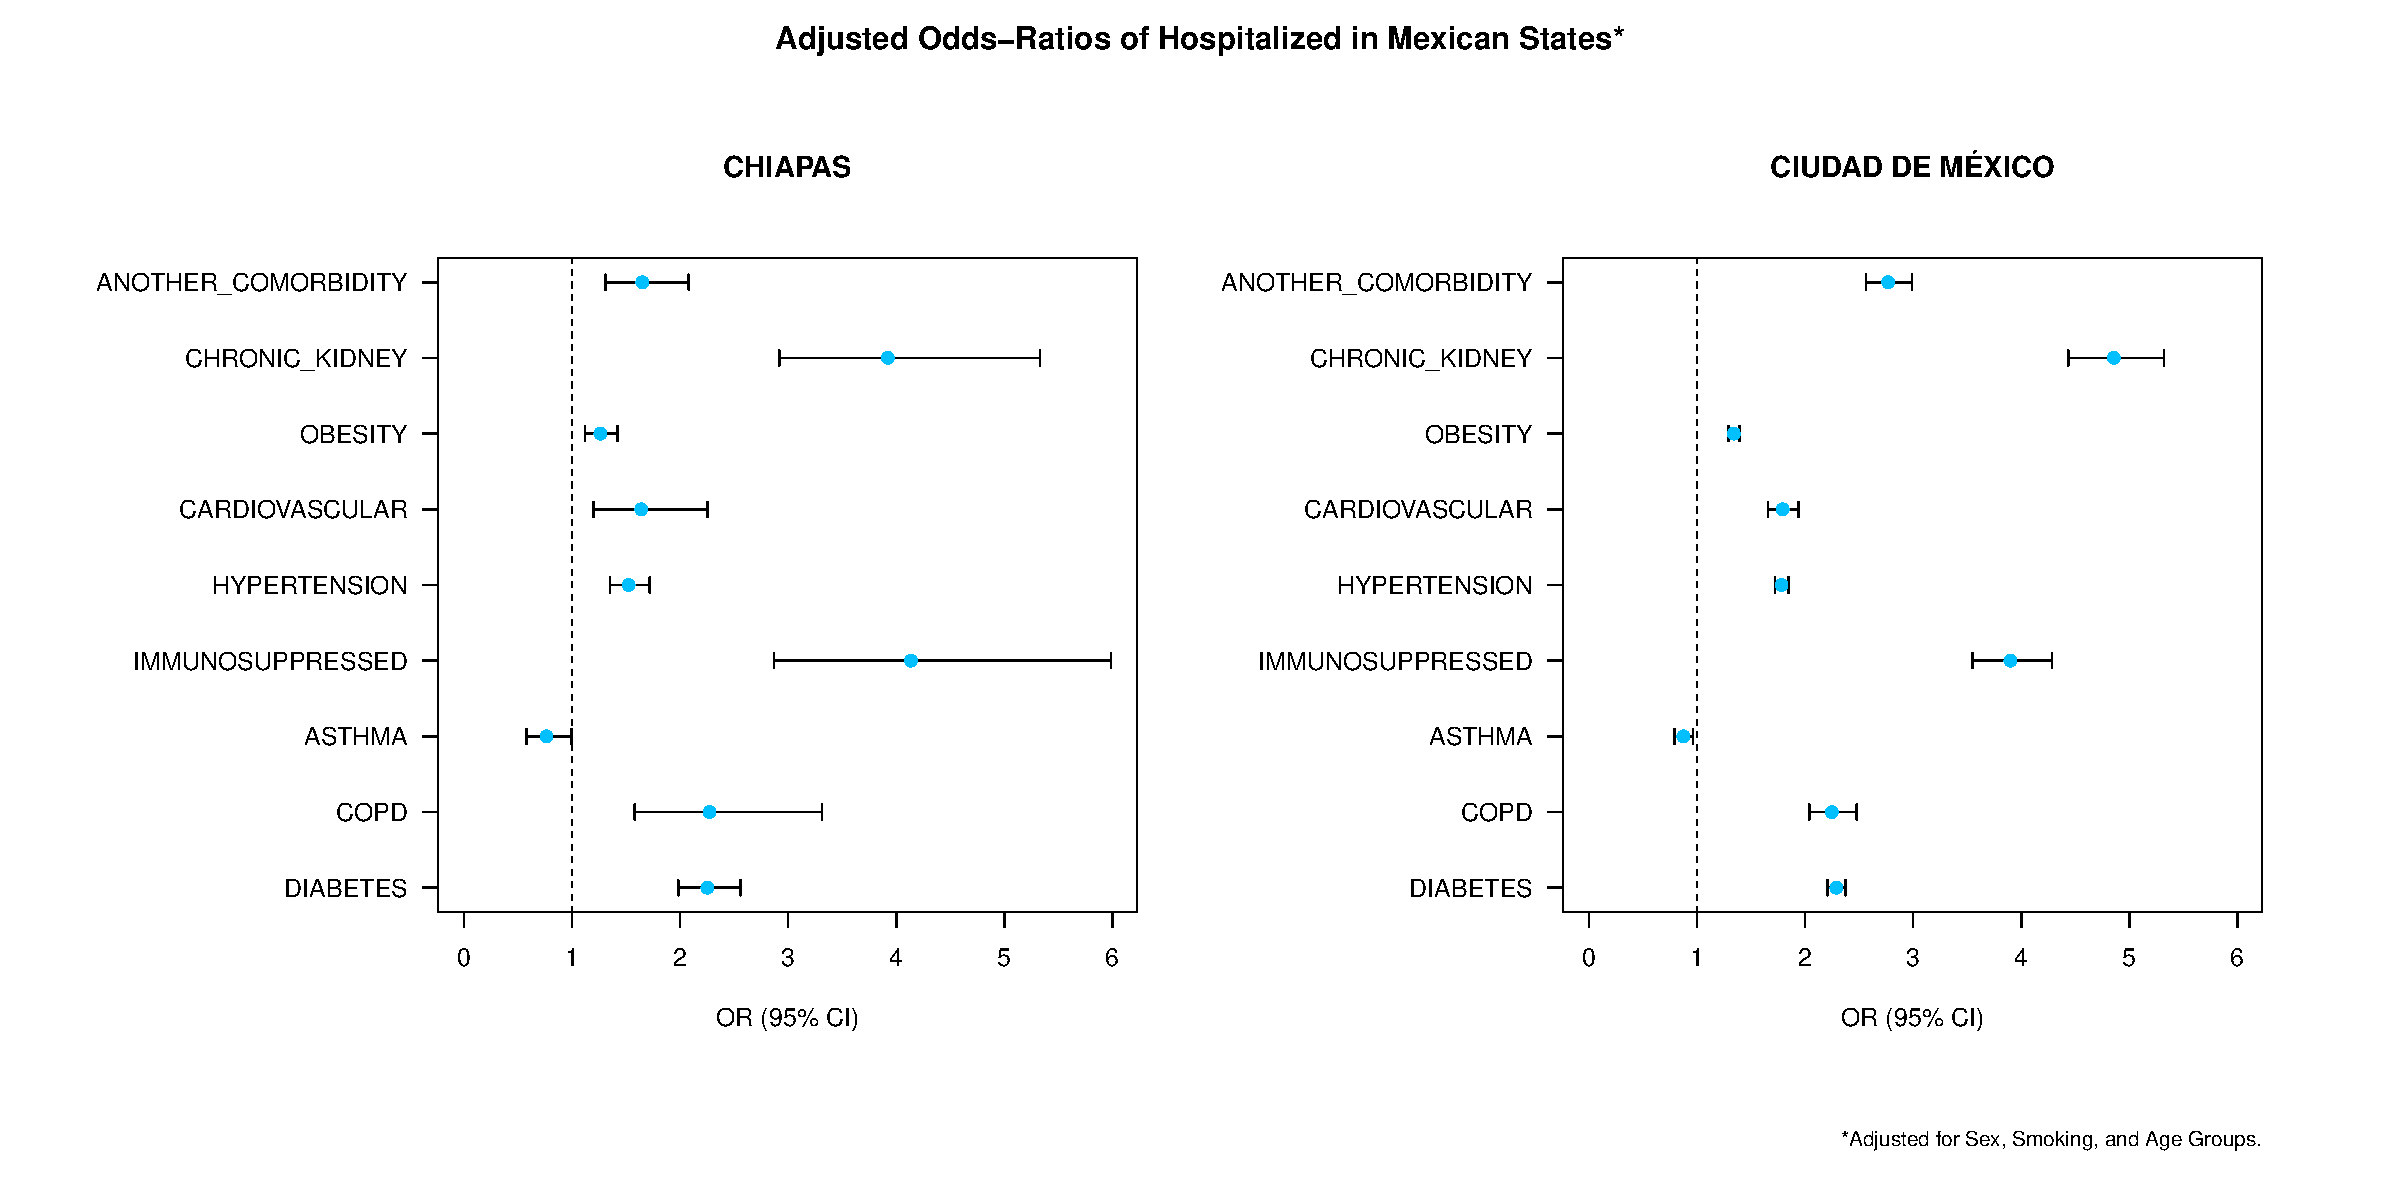
\includegraphics[width=1\linewidth]{/Users/estfernandez/Desktop/COVID-19 Comorbidities Data Analysis/figures/Case_Study_LR_Adjusted_Hospitalized} \end{center}
\end{frame}

\begin{frame}{Odds-Ratios Table}
\protect\hypertarget{odds-ratios-table-2}{}
\begin{longtable}[]{@{}lrrrr@{}}
\caption{Odds-ratios table for Chiapas.}\tabularnewline
\toprule
& exp(coef) & lower .95 & upper .95 &
Pr(\textgreater\textbar z\textbar)\tabularnewline
\midrule
\endfirsthead
\toprule
& exp(coef) & lower .95 & upper .95 &
Pr(\textgreater\textbar z\textbar)\tabularnewline
\midrule
\endhead
DIABETES & 2.253 & 1.983 & 2.559 & 0.000\tabularnewline
COPD & 2.273 & 1.581 & 3.314 & 0.000\tabularnewline
ASTHMA & 0.765 & 0.582 & 0.995 & 0.050\tabularnewline
IMMUNOSUPPRESSED & 4.136 & 2.867 & 5.988 & 0.000\tabularnewline
HYPERTENSION & 1.524 & 1.351 & 1.719 & 0.000\tabularnewline
CARDIOVASCULAR & 1.641 & 1.198 & 2.254 & 0.002\tabularnewline
OBESITY & 1.263 & 1.121 & 1.423 & 0.000\tabularnewline
CHRONIC\_KIDNEY & 3.923 & 2.918 & 5.330 & 0.000\tabularnewline
ANOTHER\_COMORBIDITY & 1.651 & 1.308 & 2.080 & 0.000\tabularnewline
\bottomrule
\end{longtable}
\end{frame}

\begin{frame}{Odds-Ratios Table}
\protect\hypertarget{odds-ratios-table-3}{}
\begin{longtable}[]{@{}lrrrr@{}}
\caption{Odds-ratios table for Cuidad de México.}\tabularnewline
\toprule
& exp(coef) & lower .95 & upper .95 &
Pr(\textgreater\textbar z\textbar)\tabularnewline
\midrule
\endfirsthead
\toprule
& exp(coef) & lower .95 & upper .95 &
Pr(\textgreater\textbar z\textbar)\tabularnewline
\midrule
\endhead
DIABETES & 2.290 & 2.207 & 2.376 & 0.000\tabularnewline
COPD & 2.248 & 2.040 & 2.477 & 0.000\tabularnewline
ASTHMA & 0.874 & 0.790 & 0.965 & 0.008\tabularnewline
IMMUNOSUPPRESSED & 3.900 & 3.548 & 4.285 & 0.000\tabularnewline
HYPERTENSION & 1.783 & 1.721 & 1.847 & 0.000\tabularnewline
CARDIOVASCULAR & 1.793 & 1.655 & 1.941 & 0.000\tabularnewline
OBESITY & 1.341 & 1.293 & 1.391 & 0.000\tabularnewline
CHRONIC\_KIDNEY & 4.857 & 4.435 & 5.321 & 0.000\tabularnewline
ANOTHER\_COMORBIDITY & 2.769 & 2.562 & 2.991 & 0.000\tabularnewline
\bottomrule
\end{longtable}
\end{frame}

\end{document}
